%% LyX 2.0.6 created this file.  For more info, see http://www.lyx.org/.
%% Do not edit unless you really know what you are doing.
\documentclass[english,french]{amsbook}
\usepackage{ae,aecompl}
\usepackage[T1]{fontenc}
\usepackage[latin1]{inputenc}
\setlength{\parskip}{\smallskipamount}
\setlength{\parindent}{0pt}
\usepackage{url}
\usepackage{amsthm}
\usepackage{amstext}
\usepackage{amssymb}
\usepackage{graphicx}

\makeatletter

%%%%%%%%%%%%%%%%%%%%%%%%%%%%%% LyX specific LaTeX commands.
%% Because html converters don't know tabularnewline
\providecommand{\tabularnewline}{\\}
%% A simple dot to overcome graphicx limitations
\newcommand{\lyxdot}{.}


%%%%%%%%%%%%%%%%%%%%%%%%%%%%%% Textclass specific LaTeX commands.
\numberwithin{section}{chapter}
\numberwithin{equation}{section}
\numberwithin{figure}{section}
  \theoremstyle{definition}
  \newtheorem*{xca*}{\protect\exercisename}
  \theoremstyle{definition}
  \newtheorem*{example*}{\protect\examplename}
\theoremstyle{plain}
\newtheorem{thm}{\protect\theoremname}
  \theoremstyle{definition}
  \newtheorem{problem}[thm]{\protect\problemname}
  \theoremstyle{definition}
  \newtheorem{defn}[thm]{\protect\definitionname}
  \theoremstyle{definition}
  \newtheorem{example}[thm]{\protect\examplename}
\newenvironment{lyxcode}
{\par\begin{list}{}{
\setlength{\rightmargin}{\leftmargin}
\setlength{\listparindent}{0pt}% needed for AMS classes
\raggedright
\setlength{\itemsep}{0pt}
\setlength{\parsep}{0pt}
\normalfont\ttfamily}%
 \item[]}
{\end{list}}
 \theoremstyle{definition}
 \newtheorem*{defn*}{\protect\definitionname}
  \theoremstyle{definition}
  \newtheorem{xca}[thm]{\protect\exercisename}
  \theoremstyle{plain}
  \newtheorem*{prop*}{\protect\propositionname}
  \theoremstyle{remark}
  \newtheorem*{rem*}{\protect\remarkname}
  \theoremstyle{plain}
  \newtheorem*{thm*}{\protect\theoremname}
  \theoremstyle{definition}
  \newtheorem*{problem*}{\protect\problemname}
  \theoremstyle{remark}
  \newtheorem{rem}[thm]{\protect\remarkname}
  \theoremstyle{plain}
  \newtheorem{prop}[thm]{\protect\propositionname}

%%%%%%%%%%%%%%%%%%%%%%%%%%%%%% User specified LaTeX commands.
\newcommand{\N}{\mathbb{N}}
\newcommand{\Z}{\mathbb{Z}}
\newcommand{\Q}{\mathbb{Q}}
\newcommand{\R}{\mathbb{R}}
\newcommand{\C}{\mathbb{C}}
\usepackage{hyperref}

\newcommand{\solution}{ \vspace{2cm}}
% Bug fix: without forcing the switch to francais after \begin{document}, chapter, table of contents and others are not translated properly
\AtBeginDocument{
\selectlanguage{francais}
}

\makeatother

\usepackage{babel}
\makeatletter
\addto\extrasfrench{%
   \providecommand{\og}{\leavevmode\flqq~}%
   \providecommand{\fg}{\ifdim\lastskip>\z@\unskip\fi~\frqq}%
}

\makeatother
  \addto\captionsenglish{\renewcommand{\definitionname}{Definition}}
  \addto\captionsenglish{\renewcommand{\examplename}{Example}}
  \addto\captionsenglish{\renewcommand{\exercisename}{Exercise}}
  \addto\captionsenglish{\renewcommand{\problemname}{Problem}}
  \addto\captionsenglish{\renewcommand{\propositionname}{Proposition}}
  \addto\captionsenglish{\renewcommand{\remarkname}{Remark}}
  \addto\captionsenglish{\renewcommand{\theoremname}{Theorem}}
  \addto\captionsfrench{\renewcommand{\definitionname}{Définition}}
  \addto\captionsfrench{\renewcommand{\examplename}{Exemple}}
  \addto\captionsfrench{\renewcommand{\exercisename}{Exercice}}
  \addto\captionsfrench{\renewcommand{\problemname}{Problème}}
  \addto\captionsfrench{\renewcommand{\propositionname}{Proposition}}
  \addto\captionsfrench{\renewcommand{\remarkname}{Remarque}}
  \addto\captionsfrench{\renewcommand{\theoremname}{Théorème}}
  \providecommand{\definitionname}{Définition}
  \providecommand{\examplename}{Exemple}
  \providecommand{\exercisename}{Exercice}
  \providecommand{\problemname}{Problème}
  \providecommand{\propositionname}{Proposition}
  \providecommand{\remarkname}{Remarque}
  \providecommand{\theoremname}{Théorème}
\providecommand{\theoremname}{Théorème}

\begin{document}

\title{Cours de Recherche Opérationnelle\\
IUT d'Orsay}


\author{Nicolas M. THIÉRY}


\email{Nicolas.Thiery@u-psud.fr}


\urladdr{http://Nicolas.Thiery.name/}

\maketitle

\chapter{Introduction à l'optimisation}


\section{TD: Ordonnancement par la méthode des potentiels}
\begin{xca*}
On veut construire une maison, ce qui consiste en $9$ tâches, le
plus rapidement possible, avec les contraintes suivantes:
\begin{itemize}
\item Certaines tâches dépendent d'autres tâches
\item Toutes les tâches demandent une semaine de travail.
\item Chaque ouvrier ne peut travailler que sur une tâche par jour
\item Il n'y a pas de gain de temps si plusieurs ouvriers travaillent sur
la même tâche
\end{itemize}
\end{xca*}
\vspace{0.3cm}


\begin{center}
\includegraphics{maison}
\par\end{center}

\vspace{0.3cm}

\begin{example*}
Organisez un emploi du temps pour un ouvrier, de façon à construire
la maison le plus rapidement.

\begin{tabular}{|c|c|c|c|c|c|c|c|}
\hline 
 & \selectlanguage{english}%
semaine 1\selectlanguage{french}%
 & \selectlanguage{english}%
semaine 2\selectlanguage{french}%
 & \selectlanguage{english}%
semaine 3\selectlanguage{french}%
 & \selectlanguage{english}%
semaine 4\selectlanguage{french}%
 & \selectlanguage{english}%
semaine 5\selectlanguage{french}%
 & \selectlanguage{english}%
semaine 6\selectlanguage{french}%
 & \selectlanguage{english}%
semaine 7\selectlanguage{french}%
\tabularnewline
\hline 
\hline 
\selectlanguage{english}%
ouvrier 1\selectlanguage{french}%
 &  &  &  &  &  &  & \tabularnewline
\hline 
\end{tabular}

De même, s'il y a deux ouvriers:

\begin{tabular}{|c|c|c|c|c|c|c|c|}
\hline 
 & \selectlanguage{english}%
semaine 1\selectlanguage{french}%
 & \selectlanguage{english}%
semaine 2\selectlanguage{french}%
 & \selectlanguage{english}%
semaine 3\selectlanguage{french}%
 & \selectlanguage{english}%
semaine 4\selectlanguage{french}%
 & \selectlanguage{english}%
semaine 5\selectlanguage{french}%
 & \selectlanguage{english}%
semaine 6\selectlanguage{french}%
 & \selectlanguage{english}%
semaine 7\selectlanguage{french}%
\tabularnewline
\hline 
\hline 
\selectlanguage{english}%
ouvrier 1\selectlanguage{french}%
 &  &  &  &  &  &  & \tabularnewline
\hline 
\selectlanguage{english}%
ouvrier 2\selectlanguage{french}%
 &  &  &  &  &  &  & \tabularnewline
\hline 
\end{tabular}

De même, s'il y a trois ouvriers:

\begin{tabular}{|c|c|c|c|c|c|c|c|}
\hline 
 & semaine 1 & \selectlanguage{english}%
semaine 2\selectlanguage{french}%
 & \selectlanguage{english}%
semaine 3\selectlanguage{french}%
 & \selectlanguage{english}%
semaine 4\selectlanguage{french}%
 & \selectlanguage{english}%
semaine 5\selectlanguage{french}%
 & \selectlanguage{english}%
semaine 6\selectlanguage{french}%
 & \selectlanguage{english}%
semaine7\selectlanguage{french}%
\tabularnewline
\hline 
\hline 
\selectlanguage{english}%
ouvrier 1\selectlanguage{french}%
 &  &  &  &  &  &  & \tabularnewline
\hline 
\selectlanguage{english}%
ouvrier 2\selectlanguage{french}%
 &  &  &  &  &  &  & \tabularnewline
\hline 
\selectlanguage{english}%
ouvrier 3\selectlanguage{french}%
 &  &  &  &  &  &  & \tabularnewline
\hline 
\end{tabular}

Et s'il y a plus d'ouvriers ?
\end{example*}
Généralisation avec des durées.


\section{Problèmes d'optimisation}
\begin{problem}
Quelles sont les coordonnées du point culminant du massif de la Chartreuse?

\includegraphics[width=1\columnwidth]{Chartreuse}

Modélisation:\end{problem}
\begin{defn}
Un \emph{problème d'optimisation} est décrit par:
\begin{itemize}
\item Un \emph{domaine} $S$ \\
Ici, $S$ est l'ensemble des points $p$ de la surface de la terre,
décrits par leur coordonnées (longitude, latitude).\\
Un élément de $S$ est appellé \emph{solution}.
\item Des contraintes $C$ définissant un sous-ensemble de $S$. \\
Ici, $C(p):=\texttt{« \ensuremath{p} est dans le massif de la Chartreuse »}$.
\\
Une solution $p$ vérifiant les contraintes $C(p)$ est dite \emph{solution
faisable}.
\item Une \emph{fonction objectif} : $z:S\mapsto\mathbb{R}$\\
Ici la fonction $p\mapsto z(p)$ qui associe à un point $p$ de la
surface de la terre sont altitude $z(p)$.
\end{itemize}
Il faut de plus préciser s'il s'agit d'un problème de \emph{maximisation}
ou de \emph{minimisation}.

Une solution faisable $p$ est dite \emph{optimale} si $z(p)\geq z(q)$
pour toute autre solution faisable $q$.

But: déterminer l'ensemble des solutions optimales.\end{defn}
\begin{example}
Modéliser les problèmes suivants, puis les résoudre ou proposer des
méthodes de résolution:
\begin{enumerate}
\item Calcul du plus court chemin dans un graphe.
\item Recherche d'un ordonnancement optimal pour ...
\item Déterminer le plus petits nombre de cartons nécessaires pour un déménagement.
\item Chercher un mat en un minimum de coup
\item Recherche de l'élément maximal d'un tableau de $n$ valeurs aléatoires.
\item Maximiser $z$ pour $z$ dans $[0,1[$.
\item Maximiser $z$ pour $z$ dans $\mathbb{R}^{+}$.
\item Déterminer la valeur minimale de la fonction $x^{2}+2x-4$.\\
\texttt{plotfunc2d(x\textasciicircum{}2 + 2{*}x - 4)}
\item Déterminer la valeur minimale de la fonction $2x^{3}-5x^{2}-x+7$.\\
\texttt{plotfunc2d(2{*}x\textasciicircum{}3 - 5{*}x - x + 7)}
\item Déterminer la valeur maximale de la fonction $\sin(x)\sin(\pi x+2)+0.01x^{2}$.\\
\texttt{plotfunc2d(sin(x) {*} sin(PI{*}x+2)-0.01{*}x\textasciicircum{}2,x=-20..20)}
\item Quelle est la profondeur maximale de l'océan?
\end{enumerate}
\end{example}
Bilan: un problème d'optimisation peut avoir
\begin{itemize}
\item Aucune solution
\item Aucune solution optimale (non borné)
\item Une unique solution optimale
\end{itemize}
Quelques méthodes d'optimisation:
\begin{enumerate}
\item Méthodes globales:

\begin{itemize}
\item Monte-Carlo
\item Recherche exhaustive (toujours possible pour un problème discret fini;
parfois la seule méthode existante)
\item Recherche exhaustive structurée, avec coupures de branches.
\end{itemize}
\item Méthodes locales, itératives:\\
Lorsque le problème a une propriété de «convexité», l'optimisation
locale amène à une optimisation globale!

\begin{itemize}
\item Algorithmes gloutons
\item Méthodes analytiques (gradient)
\item Méthode du simplexe
\end{itemize}
\item Méthodes mixtes:

\begin{itemize}
\item Monte-Carlo + gradient
\item Recuit simulé, \ldots{}
\end{itemize}
\end{enumerate}

\chapter{Programmation linéaire}


\section{Rappel d'algèbre linéaire}
\begin{problem}
Considérons le système suivant:
\begin{lyxcode}
5~~=~s1~~~~~~~+~2{*}x1~+~3{*}x2~+~~~x3

11~=~~~~s2~~~~+~4{*}x1~+~~~x2~+~2{*}x3

8~~=~~~~~~~s3~+~3{*}x1~+~4{*}x2~+~2{*}x3
\end{lyxcode}
Que peut-on dire d

$1+\frac{1+\pi}{\sqrt{1+\frac{}{}}}$

essus?















C'est un système \emph{linéaire} à 6 inconnues et 3 équations.

On peut décrire l'ensemble des solutions en prenant comme paramètres
\texttt{x1}, \texttt{x2} et \texttt{x3}.

En effet, vu sa forme triangulaire, s1, s2 et s3 s'expriment en fonction
de \texttt{x1}, \texttt{x2} et \texttt{x3}.

Transformer le système pour prendre comme paramètres $ $\texttt{s1},
\texttt{s2}, et \texttt{x1}.
\end{problem}

\section{Qu'est-ce que la programmation linéaire}


\subsection{Exemple: le problème du régime de Polly \cite[p.3]{Chvatal_LP}}
\begin{itemize}
\item Besoins journaliers:

\begin{description}
\item [{Énergie}] 2000 kcal
\item [{Protéines}] 55g
\item [{Calcium}] 800 mg
\end{description}
\item Nourriture disponible


\begin{tabular}{|c|c|c|c|c|c|}
\hline 
 & Portion & Énergie (kcal) & Protéines (g) & Calcium (mg) & Prix/portion\tabularnewline
\hline 
\hline 
Céréales & 28g & 110 & 4 & 2 & 3\tabularnewline
\hline 
Poulet & 100g & 205 & 32 & 12 & 24\tabularnewline
\hline 
Oeufs & 2 gros & 160 & 13 & 54 & 13\tabularnewline
\hline 
Lait entier & 237cc & 160 & 8 & 285 & 9\tabularnewline
\hline 
Tarte & 170g & 420 & 4 & 22 & 20\tabularnewline
\hline 
Porc et haricots & 260g & 260 & 14 & 80 & 19\tabularnewline
\hline 
\end{tabular}

\item Contraintes:

\begin{description}
\item [{Céréales}] au plus 4 portions par jour
\item [{Poulet}] au plus 3 portions par jour
\item [{Oeufs}] au plus 2 portions par jour
\item [{Lait}] au plus 8 portions par jour
\item [{Tarte}] au plus 2 portions par jour
\item [{Porc~et~haricots}] au plus 2 portions par jour
\end{description}
\end{itemize}
\begin{problem}
Polly peut-elle trouver une solution ?

Comment formaliser le problème ? (modélisation)

Qu'est-ce qui fait la spécificité du problème ?

Savez-vous résoudre des problèmes similaires ?
\end{problem}









\subsection{Forme standard d'un problème de programmation linéaire}
\begin{problem}
\cite[p. 5]{Chvatal_LP}
\begin{lyxcode}
Maximiser:~~~~~~~~~~~~5{*}x1~+~4{*}x2~+~3{*}x3

Sous~les~contraintes:~2{*}x1~+~3{*}x2~+~~~x3~<=~~5~

~~~~~~~~~~~~~~~~~~~~~~4{*}x1~+~~~x2~+~2{*}x3~<=~11

~~~~~~~~~~~~~~~~~~~~~~3{*}x1~+~4{*}x2~+~2{*}x3~<=~~8

~~~~~~~~~~~~~~~~~~~~~~x1,~x2,~x3~>=~0



Minimiser:~~~~~~~~~~~~3{*}x1~-~~~x2

Sous~les~contraintes:~-~x1~+~6{*}x2~-~~~x3~+~~~x4~>=~-3~

~~~~~~~~~~~~~~~~~~~~~~~~~~~~~7{*}x2~~~~~~~~+~2{*}x4~=~~~5

~~~~~~~~~~~~~~~~~~~~~~~~x1~+~~~x2~+~~~x3~~~~~~~~=~~~1

~~~~~~~~~~~~~~~~~~~~~~~~~~~~~~~~~~~~~~x3~+~~~x4~<=~~2

~~~~~~~~~~~~~~~~~~~~~~~x2,~x3~>=~0
\end{lyxcode}
\end{problem}
\begin{defn*}
Problème de programmation linéaire sous \emph{forme standard:}

Maximiser:

\[
z:=\sum_{j=1}^{n}c_{j}x_{j}
\]


Sous les contraintes:

\[
\sum_{j=1}^{n}a_{ij}x_{j}\leq b_{i},\textrm{ pour }i=1,\ldots,m
\]
 

\[
x_{j}\geq0,\textrm{ pour }j=1,\ldots,n
\]


Un choix des valeurs des variables $(x_{1},\ldots,x_{n})$ est appelé
\emph{solution} du problème.

Une solution est \emph{faisable} si elle vérifie les contraintes.

$z$ est appelé \emph{fonction objective}. À chaque solution elle
associe une valeur.

Une solution est \emph{optimale} si elle est faisable et maximize
la fonction objective.\end{defn*}
\begin{xca}
Peut-on mettre sous forme standard les exemples précédents ?
\end{xca}

\subsection{Existence de solutions optimales ?}
\begin{problem}
\cite[p. 7]{Chvatal_LP} On considère les trois problèmes de programmation
linéaire standard suivants, écrits avec la syntaxe du système de calcul
formel \texttt{MuPAD}:
\begin{lyxcode}
Chvatal7a~:=~{[}~{[}~~~x1~~~~~~<=~3,~

~~~~~~~~~~~~~~~~~~~~~~~~x2~<=~7~{]},

~~~~~~~~~~~~~~~~3~+x1~~+x2,~

~~~~~~~~~~~~~~~NonNegative{]}:

Chvatal7b~:=~{[}~{[}~~~x1~~+x2~<=~2,~

~~~~~~~~~~~~~~~~-2{*}x1-2{*}x2~<=~-10~{]},

~~~~~~~~~~~~~~~~~3{*}x1~~-x2,~

~~~~~~~~~~~~~~~NonNegative{]}:~

Chvatal7c~:=~{[}~{[}-2{*}x1~~+x2~<=~-1,~

~~~~~~~~~~~~~~~~~~-x1-2{*}x2~<=~-2~{]},

~~~~~~~~~~~~~~~~~~~x1~~-x2,

~~~~~~~~~~~~~~~NonNegative{]}:

extra~~~~~:=~{[}~{[}~~~x1~~+x2~<=~1~{]},

~~~~~~~~~~~~~~~~~~~x1~~+x2,

~~~~~~~~~~~~~~~NonNegative{]}:
\end{lyxcode}
\end{problem}
\begin{lyxcode}
\end{lyxcode}
\begin{problem}
Déterminer pour ces trois problèmes s'il y a des solutions optimales.\end{problem}
\begin{lyxcode}






\solution\end{lyxcode}
\begin{itemize}
\item Premier cas: une solution optimale unique
\item Deuxième cas: pas de solution faisable
\item Troisième cas: pas de solution optimale, car on peut faire tendre
la fonction objective vers l'infini avec des solutions faisables.
\item Quatrième cas: une infinité de solutions optimales.
\end{itemize}

\section{Algorithme du simplexe}


\subsection{Premier problème}
\begin{problem}
\label{probleme:simplexe1}\cite[p. 13]{Chvatal_LP}
\begin{lyxcode}
Chvatal13~:=~{[}\{2{*}x1~+~3{*}x2~+~~~x3~<=~5,~

~~~~~~~~~~~~~~~4{*}x1~+~~~x2~+~2{*}x3~<=~11,~

~~~~~~~~~~~~~~~3{*}x1~+~4{*}x2~+~2{*}x3~<=~8~~\},~

~~~~~~~~~~~~~~~5{*}x1~+~4{*}x2~+~3{*}x3,~

~~~~~~~~~~~~~~NonNegative{]}:
\end{lyxcode}
\end{problem}
Solution faisable ?

Amélioration de la solution ?














\solution

Introduction de variables d'écart:
\begin{lyxcode}
5~~=~s1~~~~~~~+~2{*}x1~+~3{*}x2~+~~~x3

11~=~~~~s2~~~~+~4{*}x1~+~~~x2~+~2{*}x3

8~~=~~~~~~~s3~+~3{*}x1~+~4{*}x2~+~2{*}x3

-{}-{}-{}-{}-{}-{}-{}-{}-{}-{}-{}-{}-{}-{}-{}-{}-{}-{}-{}-{}-{}-{}-{}-{}-{}-{}-{}-{}-{}-{}-{}-{}-{}-

z~~=~~~~~~~~~~~~5{*}x1~+~4{*}x2~+~3{*}x3
\end{lyxcode}
En augmentant \texttt{x1} jusqu'à $5/2$, on fait tomber \texttt{s1}
à zéro.

On transforme le système, pour se ramener à une situation similaire
à la précédente:
\begin{lyxcode}
5/2~=~x1~~~~~~~+~3/2{*}x2~+~1/2{*}x3~+~1/2{*}s1

1~~~=~~~~s2~~~~-~~~5{*}x2~~~~~~~~~~~~-~2{*}s1

1/2~=~~~~~~~s3~-~1/2{*}x2~+~1/2{*}x3~-~3/2{*}s1

-{}-{}-{}-{}-{}-{}-{}-{}-{}-{}-{}-{}-{}-{}-{}-{}-{}-{}-{}-{}-{}-{}-{}-{}-{}-{}-{}-{}-{}-{}-{}-{}-{}-{}-{}-{}-{}-{}-{}-{}-

z~~~=~25/2~~~~~-~7/2~x2~+~1/2{*}x3~-~5/2{*}s1
\end{lyxcode}
On augmente x3 jusqu'à 1, ce qui fait tomber s3 à 0:
\begin{lyxcode}
1~=~x3~~~~~~~-~~~x2~-~3{*}s1~+~2{*}s3

2~=~~~~x1~~~~+~2{*}x2~+~2{*}s1~-~~~s3

1~=~~~~~~~s2~-~5{*}x2~-~2{*}s1

-{}-{}-{}-{}-{}-{}-{}-{}-{}-{}-{}-{}-{}-{}-{}-{}-{}-{}-{}-{}-{}-{}-{}-{}-{}-{}-{}-{}-{}-{}-{}-{}-

z~=~13~~~~~~~-~3{*}x2~-~~~s1~-~~~s3
\end{lyxcode}
Et maintenant, que fait-on ?


\subsection{Tableaux}
\begin{problem}
\cite[p. 19]{Chvatal_LP}
\begin{lyxcode}
Chvatal19~:=~{[}{[}~~x1~+~3{*}x2~~~+~x3~<=~3,~

~~~~~~~~~~~~~~~~-x1~~~~~~~~~+3{*}x3~<=~2,

~~~~~~~~~~~~~~~2{*}x1~+~3{*}x2~~~-~x3~<=~2,~

~~~~~~~~~~~~~~~2{*}x1~~~-~x2~+~2{*}x3~<=~4{]},~

~~~~~~~~~~~~~~~5{*}x1~+~5{*}x2~+~3{*}x3,~

~~~~~~~~~~~~~~NonNegative{]}:
\end{lyxcode}
\end{problem}
\begin{defn*}
\emph{Tableau initial:}

\[
b_{i}=s_{i}+\sum_{j=1}^{n}a_{ij}x_{j},\textrm{ pour }i=1,\ldots,m
\]


\[
z=\sum_{j=1}^{n}c_{j}x_{j}
\]


Ou sous forme matricielle:
\begin{eqnarray*}
B & = & S+AX\\
z & = & CX\\
X & \geq & 0
\end{eqnarray*}
\end{defn*}
\begin{example*}
Tableau initial du problème précédent:
\begin{lyxcode}
3~=~s1~~~~~~~~~+~x1~+~3~x2~~~+~x3

2~=~~~s2~~~~~~~-~x1~~~~~~~~+~3~x3

2~=~~~~~s3~~~+~2~x1~+~3~x2~~~-~x3

4~=~~~~~~~s4~+~2~x1~~~-~x2~+~2~x3

-{}-{}-{}-{}-{}-{}-{}-{}-{}-{}-{}-{}-{}-{}-{}-{}-{}-{}-{}-{}-{}-{}-{}-{}-{}-{}-{}-{}-{}-{}-{}-{}-

z~=~0~~~~~~~~+~5~x1~+~5~x2~+~3~x3
\end{lyxcode}
\end{example*}
\begin{example}
On peut l'abréger sous forme matricielle: 
\begin{lyxcode}
read(\textquotedbl{}tableaux.mu\textquotedbl{}):

linopt::Transparent(Chvatal19);

+-~~~~~~~~~~~~~~~~~~~~~~~~~~~~~~~~~~~~~~~~~~~~~~~~~~~-+

|\textquotedbl{}linopt\textquotedbl{},\textquotedbl{}restr\textquotedbl{},slk{[}1{]},slk{[}2{]},slk{[}3{]},slk{[}4{]},x3,x1,x2|

|~~~~~~~~~~~~~~~~~~~~~~~~~~~~~~~~~~~~~~~~~~~~~~~~~~~~~|

|~~\textquotedbl{}obj\textquotedbl{},~~~~0,~~~~~~0,~~~~~0,~~~~~0,~~~~~0,~~~3,~5,~5|

|~~~~~~~~~~~~~~~~~~~~~~~~~~~~~~~~~~~~~~~~~~~~~~~~~~~~~|

|~slk{[}1{]},~~~~3,~~~~~~1,~~~~~0,~~~~~0,~~~~~0,~~~1,~1,~3|

|~~~~~~~~~~~~~~~~~~~~~~~~~~~~~~~~~~~~~~~~~~~~~~~~~~~~~|

|~slk{[}2{]},~~~~2,~~~~~~0,~~~~~1,~~~~~0,~~~~~0,~~~3,-1,~0|

|~~~~~~~~~~~~~~~~~~~~~~~~~~~~~~~~~~~~~~~~~~~~~~~~~~~~~|

|~slk{[}3{]},~~~~2,~~~~~~0,~~~~~0,~~~~~1,~~~~~0,~~-1,~2,~3|

|~~~~~~~~~~~~~~~~~~~~~~~~~~~~~~~~~~~~~~~~~~~~~~~~~~~~~|

|~slk{[}4{]},~~~~4,~~~~~~0,~~~~~0,~~~~~0,~~~~~1,~~~2,~2,-1|

+-~~~~~~~~~~~~~~~~~~~~~~~~~~~~~~~~~~~~~~~~~~~~~~~~~~~-+
\end{lyxcode}
\end{example}
\begin{defn*}
De manière générale, un \emph{tableau} est un ensemble d'équations
de la forme:
\begin{lyxcode}
4~=~x1~~~~~~~+~3/2~x2~~-~1/2~x3~+~1/2~s4~

2~=~~~s1~~~~~+~3/2~x2~~+~3/2~x3~-~1/2~s4~

3~=~~~~~s2~~~+~3/2~x2~~+~5/2~x3~+~1/2~s4~

2~=~~~~~~~s3~~~-~4~x2~~~~+~3~x3~~~~~-~s4~

-{}-{}-{}-{}-{}-{}-{}-{}-{}-{}-{}-{}-{}-{}-{}-{}-{}-{}-{}-{}-{}-{}-{}-{}-{}-{}-{}-{}-{}-{}-{}-{}-{}-{}-{}-{}-{}-{}-{}-~

z~=~5~~~~~~~~-~5/2~x2~+~11/2~x3~-~5/2~s4
\end{lyxcode}
$x_{1},s_{1},s_{2},s_{3}$ sont les variables \emph{basiques;} $\{x_{1},s_{1},s_{2},s_{3}\}$
est la \emph{base}.

$x_{2},x_{3},s_{4}$ sont les variables \emph{non basiques.}\end{defn*}
\begin{defn}
Le point de coordonnées $(0,\ldots,0)$ dans les variables non-basiques
est appellé \emph{solution basique} du tableau.

Un tableau est \emph{faisable} si la solution basique $(0,\ldots,0)$
est une solution faisable.

De manière équivalente, un tableau est faisable si les constantes
dans les équations du haut sont toutes positives ou nulles.
\end{defn}
Revenons à l'exemple \cite[p. 19]{Chvatal_LP}:
\begin{lyxcode}
read(\textquotedbl{}tableaux.mu\textquotedbl{}):

t:=linopt::Transparent(Chvatal19);

t:=linopt::Transparent::userstep(t,~slk{[}3{]},~x3);\end{lyxcode}
\begin{xca}
\cite[2.1 p. 26]{Chvatal_LP}

Utilisez l'algorithme du simplexe pour résoudre les programmes linéaires
suivants:
\begin{lyxcode}
Chvatal26\_21a~:=

{[}{[}~~x1~~+x2+2{*}x3~<=~4,

~~2{*}x1~~~~~+3{*}x3~<=~5,

~~2{*}x1~~+x2+3{*}x3~<=~7{]},

~~3{*}x1+2{*}x2+4{*}x3,

~NonNegative{]}:



Chvatal26\_21c~:=

{[}{[}2{*}x1+3{*}x2~<=~3,

~~~~x1+5{*}x2~<=~1,

~~2{*}x1~~+x2~<=~4,

~~4{*}x1~~+x2~<=~5{]},

~~2{*}x1~~+x2,

~NonNegative{]}:
\end{lyxcode}
\end{xca}
%
\begin{xca}
Essayez d'appliquer l'algorithme du simplexe aux programmes linéaires
de l'exercice \cite[p. 7]{Chvatal_LP} (cf. ci-dessus). Que se passe-t'il
?
\end{xca}

\section{Pièges et comment les éviter}


\subsection{Bilan des épisodes précédents}

On a un algorithme qui marche sur quelques exemples.

Il faut vérifier trois points pour savoir s'il marche en général:
\begin{enumerate}
\item Initialisation
\item Itération
\item Terminaison
\end{enumerate}

\subsection{Itération}
\begin{prop*}
Étant donné un tableau faisable, on peut toujours effectuer l'une
des opérations suivantes:\end{prop*}
\begin{enumerate}
\item Conclure que le système a une solution optimale unique, la calculer
et la certifier;
\item Conclure que le système a une infinité de solutions optimales, les
calculer et les certifier;
\item Conclure que le système est non borné, et le certifier en décrivant
une demi-droite de solutions sur laquelle $z$ prend des valeurs aussi
grandes que voulu.
\item Trouver une variable entrante, une variable sortante, et effectuer
un pivot. Par construction, le tableau obtenu est équivalent au tableau
précédent, et est encore faisable. De plus, $z$ a \emph{augmenté
au sens large} (i.e. la constante $z^{*}$ dans la nouvelle expression
de $z$ est supérieure ou égale à l'ancienne).\end{enumerate}
\begin{proof}
Il suffit d'analyser le tableau faisable. Notons $S_{1},\ldots,S_{m}$
les variables basiques, $X_{1},\ldots,X_{n}$ les variables non-basiques,
et $C_{1},\ldots,C_{n},z^{*}$ les coefficients tels que $z=z^{*}+\sum C_{i}X_{i}$. 

Par exemple, dans le tableau final du problème\ref{probleme:simplexe1},
on a $X_{1}=x_{2}$, $X_{2}=s_{1}$, $X_{3}=s_{2}$, $S_{1}=x_{1}$,
$S_{2}=x_{3}$, $S_{3}=s_{3}$, $C_{1}=-3$, $C_{2}=-1$, $C_{3}=-1$
et $z^{*}=13$.
\begin{enumerate}
\item Si $C_{i}<0$, pour tout $i$, alors la solution basique du tableau,
de coordonnées $X_{1}^{*}=\cdots=X_{n}^{*}=0$ est l'unique solution
optimale. Vérifiez le en prouvant qu'une toute solution faisable quelconque
de coordonnées $X_{1},\ldots,X_{n}$ donnant la même valeur $z=z^{*}$
à la fonction objective est égale à la solution basique du tableau.
\item Si $C_{i}\leq0$ pour tout $i$, la solution basique du tableau est
optimale, et l'ensemble des solutions optimales est décrit par les
inéquations linéaires du système et l'annulation des variables non-basiques
$X_{i}$ pour lesquelles on a $C_{i}<0$. Les détails sont similaires
au 1.
\item Sinon, on peut prendre $X_{i}$, variable non-basique avec un coefficient
$C_{i}>0$. Si les équations du tableau n'imposent pas de limite sur
$X_{i}$, le système est non borné: la demi-droite décrite par $(0,\ldots,0,X_{i},0,\ldots,0)$
pour $X_{i}\geq0$ est composée de solutions faisables qui donnent
des valeurs aussi grandes que voulu à $z$.
\item Autrement, une des variables basiques $S_{j}$ tombe à zéro, et on
peut faire un pivot entre la variable entrante $X_{i}$ et la variable
sortante $S_{j}$. Par construction, la nouvelle solution basique
correspond à une solution faisable $(0,\ldots,0,X_{i},0,\ldots,0)$
pour un $X_{i}\geq0$. En particulier le nouveau tableau est faisable,
et comme $C_{i}\geq0$, la constante $z^{*}$ a augmenté au sens large.
\end{enumerate}
\end{proof}
\begin{example*}
\cite[p. 29]{Chvatal_LP} Système où $z$ n'augmente pas strictement
lors du pivot:\end{example*}
\begin{lyxcode}
Chvatal29~:=~~{[}{[}~~~~~~~~~~~~~~2{*}x3~<=~1,~

~~~~~~~~~~~~~~~~-~x1~+~3{*}x2~+~4{*}x3~<=~2,~

~~~~~~~~~~~~~~~~2{*}x1~-~4{*}x2~+~6{*}x3~<=~3{]},

~~~~~~~~~~~~~~~~2{*}x1~~~-~x2~+~8{*}x3,~

~~~~~~~~~~~~~~~~NonNegative{]}:

t0:=~linopt::Transparent(Chvatal29);

t1:=~linopt::Transparent::userstep(t0,~slk{[}1{]},~x3);

t2:=~linopt::Transparent::userstep(t1,~slk{[}3{]},~x1);

t3:=~linopt::Transparent::userstep(t2,~slk{[}2{]},~x2);

t4:=~linopt::Transparent::userstep(t3,~x3,~slk{[}1{]});\end{lyxcode}
\begin{rem*}
Lorsque $z$ n'augmente pas, on est forcément dans une situation de
dégénérescence: le pivot change le tableau, mais pas la solution basique
décrite par le tableau.
\end{rem*}

\subsection{Terminaison}
\begin{problem}
Peut-on garantir que l'algorithme va finir par s'arrêter ?
\end{problem}
%

%

%

%

%

%

%

%

\solution
\begin{thm*}
Si l'algorithme du simplexe ne cycle pas, il termine en au plus $C(n+m,m)$
itérations.\end{thm*}
\begin{proof}
(Résumé)

Chaque itération correspond à un tableau faisable. 

Un tableau faisable est entièrement caractérisé par le choix des variables
basiques.

Il n'y a \og que \fg{} $C(n+m,m)$ choix possibles de variables
basiques.\end{proof}
\begin{rem*}
L'algorithme ne peut cycler qu'en présence de dégénérescence.
\end{rem*}
Avec une stratégie incorrecte, l'algorithme du simplexe peut cycler
éternellement:
\begin{example*}
\cite[p. 31]{Chvatal_LP} Système cyclant en 6 itérations avec la
stratégie:
\begin{itemize}
\item Choix de la variable entrante avec le coefficient dans l'expression
de $z$ le plus fort
\item Choix de la variable sortante avec le plus petit index\end{itemize}
\begin{lyxcode}
Chvatal31~:=~{[}{[}0.5{*}x1~-~5.5{*}x2~-~2.5{*}x3~+~~9{*}x4~<=~0,~

~~~~~~~~~~~~~~~0.5{*}x1~-~1.5{*}x2~-~0.5{*}x3~+~~~~x4~<=~0,

~~~~~~~~~~~~~~~~~~~x1~~~~~~~~~~~~~~~~~~~~~~~~~~~<=~1{]},

~~~~~~~~~~~~~~~~10{*}x1~~-~57{*}x2~~~-~9{*}x3~-~24{*}x4,

~~~~~~~~~~~~~~NonNegative{]}:

t0~:=~linopt::Transparent(Chvatal31);

t1~:=~linopt::Transparent::userstep(t0,~slk{[}1{]},~x1);

t2~:=~linopt::Transparent::userstep(t1,~slk{[}2{]},~x2);

t3~:=~linopt::Transparent::userstep(t2,~x1,~x3);

t4~:=~linopt::Transparent::userstep(t3,~x2,~x4);

t5~:=~linopt::Transparent::userstep(t4,~x3,~slk{[}1{]});

t6~:=~linopt::Transparent::userstep(t5,~x4,~slk{[}2{]});
\end{lyxcode}
\end{example*}
Comment garantir que l'algorithme ne cyclera pas ?
\begin{itemize}
\item Méthode des perturbations
\item La méthode du plus petit index

\begin{thm*}
L'algorithme du simplexe termine si, lorsqu'il y a ambiguïté sur le
choix de la variable entrante ou sortante, on choisit toujours la
variable de plus petit index.
\end{thm*}

Cette méthode est simple et élégante. 


Par contre, elle empêche toute stratégie pour faire converger l'algorithme
plus vite.

\item Méthodes intermédiaires
\end{itemize}

\subsection{Initialisation}

Pour le moment, l'algorithme du simplexe nécessite de partir d'un
tableau faisable.
\begin{problem*}
Dans le cas général, comment se ramener à un tableau faisable?

Le système pourrait même ne pas avoir de solution!\end{problem*}
\begin{example*}
\cite[p. 39]{Chvatal_LP} Système $P_{1}$:

Maximiser: $x_{1}-x_{2}+x_{3}$

Sous les contraintes:

$2x_{1}-x_{2}+2x_{3}\leq4$

$2x_{1}-3x_{2}+x_{3}\leq-5$

$-x_{1}+x_{2}-2x_{3}\leq-1$

$x_{1},x_{2},x_{3}\geq0$
\end{example*}
%

%

%

%

%

\solution
\begin{example*}
Introduction d'un \emph{système} auxiliaire $P_{0}$ pour déterminer
si $P$ est faisable:

Maximiser: $-x_{0}$

Sous les contraintes:

$2x_{1}-x_{2}+2x_{3}-x_{0}\leq4$

$2x_{1}-3x_{2}+x_{3}-x_{0}\leq-5$

$-x_{1}+x_{2}-2x_{3}-x_{0}\leq-1$

$x_{0},x_{1},x_{2},x_{3}\geq0$

Remarques:
\begin{itemize}
\item \emph{$P_{0}$ est faisable (prendre $x_{0}$ suffisamment grand);}
\item \emph{Les solutions faisables de $P$ correspondent aux solutions
faisables de $P_{0}$ avec $x_{0}=0$;}
\item \emph{$P$ est faisable si et seulement si $P_{0}$ a une solution
faisable avec $x_{0}=0$.}
\end{itemize}
Étudions ce nouveau système:
\begin{lyxcode}
Chvatal40~:=~{[}{[}~-x1~~~+~x2~-~2{*}x3~-~x0~<=~-1,

~~~~~~~~~~~~~~~2{*}x1~-~3{*}x2~~~+~x3~-~x0~<=~-5,~

~~~~~~~~~~~~~~~2{*}x1~~~-~x2~+~2{*}x3~-~x0~<=~4{]},~

~~~~~~~~~~~~~~-x0,~

~~~~~~~~~~~~~~NonNegative{]}:

t0:=linopt::Transparent(Chvatal40);

t1:=linopt::Transparent::userstep(t0,~slk{[}2{]},~x0);

t2:=linopt::Transparent::userstep(t1,~slk{[}1{]},~x2);

t3:=linopt::Transparent::userstep(t2,~x0,~x3);
\end{lyxcode}
Maintenant, nous savons que le système $P$ est faisable.

En fait, en éliminant $x_{0}$ on obtient même un tableau faisable
pour $P$!
\end{example*}
Algorithme du simplexe en deux phases pour résoudre un problème $P$
sous forme standard:

Phase I: 
\begin{enumerate}
\item Si $(0,\ldots,0)$ est solution faisable de $P$, on passe directement
à la phase II.
\item Définir un problème auxiliaire $P_{0}$.
\item Le premier tableau pour $P_{0}$ est infaisable.
\item Le rendre faisable par un pivot approprié de $x_{0}$. 
\item Appliquer le simplexe habituel:

\begin{enumerate}
\item Si à une étape donnée, $x_{0}$ peut sortir de la base, le faire en
priorité: 


En effet, il y a une solution faisable avec $x_{0}=0$, et on peut
passer en phase II.

\item Si à une étape donnée on atteint une solution optimale:

\begin{enumerate}
\item Si $x_{0}$ n'est pas basique: 


Il y a une solution faisable avec $x_{0}=0$. On peut donc passer
en phase II.

\item Si $x_{0}$ est basique et $z_{0}<0$: 


$P$ est infaisable, et on s'arrête.

\item Sinon $x_{0}$ est basique et $z_{0}=0$:


Situation impossible si on fait toujours sortir $x_{0}$ en priorité
de la base.

\end{enumerate}
\end{enumerate}
\item Tirer de $P_{0}$ un tableau faisable pour $P$;
\end{enumerate}
Phase II:
\begin{enumerate}
\item Appliquer le simplexe habituel à partir du tableau donné par $P_{0}$.\end{enumerate}
\begin{xca*}
\cite[ex 3.9a p. 44]{Chvatal_LP}

Maximiser $3x_{1}+x_{2}$

Sous les contraintes:

$x_{1}-x_{2}\leq-1$

$-x_{1}-x_{2}\leq-3$

$2x_{1}+x_{2}\leq4$

$x_{1},x_{2}\geq0$\end{xca*}
\begin{lyxcode}
t0:=linopt::Transparent(Chvatal44\_39a0)

t1:=linopt::Transparent::userstep(t0,~slk{[}2{]},~x0)

t2:=linopt::Transparent::userstep(t1,~slk{[}1{]},~x1)

t3:=linopt::Transparent::userstep(t2,~x0,~x2)

t0:=linopt::Transparent(Chvatal44\_39a)

t1:=linopt::Transparent::userstep(t0,~slk{[}1{]},~x1)

t2:=linopt::Transparent::userstep(t1,~slk{[}2{]},~x2)

t3:=linopt::Transparent::userstep(t2,~slk{[}3{]},~slk{[}2{]})
\end{lyxcode}

\subsection{Le théorème fondamental de la programmation linéaire}
\begin{thm*}
Tout programme linéaire $P$ sous forme standard a l'une des propriétés
suivantes:\end{thm*}
\begin{enumerate}
\item Si $P$ n'a pas de solutions optimales, alors $P$ est infaisable
ou non borné;
\item Si $P$ a une solutions faisable, alors $P$ a une solution basique
faisable;
\item Si $P$ a une solution optimale, alors $P$ a une solution basique
optimale.
\end{enumerate}

\chapter{Problèmes de flot maximum}


\section{Introduction}
\begin{defn*}
\emph{Problème de flot max:}
\begin{itemize}
\item Réseau avec source et puits
\item Pas de coûts sur les arcs
\item Contraintes de capacités sur les arcs
\item Production et consommation nulle sur chaque noeud intermédiaire
\end{itemize}

\begin{center}
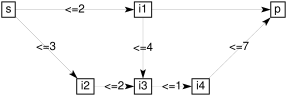
\includegraphics[width=1\columnwidth]{\lyxdot \lyxdot /\lyxdot \lyxdot /RO/Notes/flot}
\par\end{center}

Objectif: 

Maximiser le \emph{volume} du flot, c'est-à-dire la quantité transportée
entre $s$ et $p$.\end{defn*}
\begin{example*}
Un dimanche soir, maximiser le nombre de voitures allant d'Albertville
à Lyon, en les répartissant entre les différentes routes possibles.\end{example*}
\begin{xca*}
Mettre le problème de flot dessiné ci-dessus sous forme de programme
linéaire.
\end{xca*}









Clairement, cela se généralise à tout problème de flot max.
\begin{problem*}
Que peut-on en déduire ?
\end{problem*}







\begin{itemize}
\item On a un algorithme de résolution (simplexe)
\item On doit bien avoir une dualité!
\end{itemize}

\section{Coupes dans un problème de flot}
\begin{defn*}
Une \emph{coupe} $C$ dans un réseau est un ensemble de sommets du
réseau contenant la source.

La capacité de la coupe $C$ est la somme des capacités des arrêtes
sortantes de $C$.\end{defn*}
\begin{example*}
Dans notre réseau, la coupe $C=\left\{ s\right\} $ est de capacité
$5$.

\begin{center}
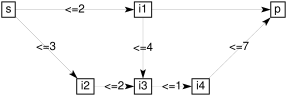
\includegraphics[width=1\columnwidth]{\lyxdot \lyxdot /\lyxdot \lyxdot /RO/Notes/flot}
\par\end{center}

\end{example*}
\begin{xca*}
Quelle est la capacité de la coupe $C=\left\{ s,i_{2},i_{3}\right\} $?

Que peut-on en déduire sur la valeur d'un flot ?
\end{xca*}










\solution
\begin{prop*}
Pour toute coupe $C$ et tout flot $F$ dans un réseau, la capacité
$\left|C\right|$ de la coupe est supérieure au volume $\left|F\right|$
du flot: $\left|C\right|\geq\left|F\right|$.\end{prop*}
\begin{xca*}
Chercher un flot maximal et une coupe minimal dans notre exemple?

Que peut-on dire?
\end{xca*}

\section{Algorithme de Ford-Fulkerson}

Nous allons maintenant donner un algorithme qui permet de calculer
un flot maximal.

Mieux, comme l'algorithme du simplexe, cet algorithme va donner des
résultats théoriques!
\begin{example*}
On veut transporter le plus grand nombre possible de voyageurs de
San-Francisco à New-York, sachant qu'il ne reste que quelques places
dans les avions entre les villes suivantes:

\begin{center}
\includegraphics[width=1\columnwidth]{\lyxdot \lyxdot /\lyxdot \lyxdot /RO/Notes/flot-voyageurs}
\par\end{center}

\end{example*}
\begin{defn*}
Soit $R$ un réseau, et $F$ un flot donné dans ce réseau.

Un chemin allant de la source $s$ au puits $p$ est \emph{$F$-augmentant}
si pour chaque arête $ij$ du chemin on a:
\begin{itemize}
\item $x_{ij}<u_{ij}$ si l'arc $ij$ est dans le même sens que dans le
réseau
\item $x_{ij}>0$ si l'arc $ij$ est dans le sens inverse du réseau.
\end{itemize}
\end{defn*}
À partir d'un chemin $F$-augmentant, on peut construire un nouveau
flot $F'$ qui sera de volume strictement plus gros.

Le principe de l'algorithme de Ford-Fulkerson est de partir d'un flot
$F$ quelconque, et de l'améliorer itérativement en recherchant des
chemins $F$-augmentant.

À chaque étape, la recherche d'un chemin $F$-augmentant se fait par
un parcours en profondeur, de manière similaire à la recherche d'un
chemin $M$-augmentant dans un graphe biparti. Si cette recherche
échoue, elle dévoile une coupe de capacité égale au flot, ce qui donne
un certificat d'optimalité du flot.
\begin{rem}
On peut toujours initialiser l'algorithme avec un flot nul.

Si toutes les capacités sont entières et finies, chaque itération
augmente le flot d'au moins $1$. Cet algorithme ne peut donc pas
cycler, et il termine en un nombre fini d'étapes.

Avec une mauvaise stratégie, et des capacités infinies ou non-entières,
l'algorithme peut ne pas terminer.

\includegraphics[width=0.5\columnwidth]{\lyxdot \lyxdot /\lyxdot \lyxdot /RO/Notes/flot-mauvais}

Avec une stratégie convenable, cet algorithme est en fait polynomial,
en $O\left(n^{3}\right)$, même si les capacités sont infinies ou
non entières.

Pour les réseaux avec peu d'arcs, il y a des algorithmes plus compliqués
qui permettent d'obtenir d'encore meilleurs bornes. Cf. \cite[p.~369]{Chvatal_LP}
pour les détails.
\end{rem}

\section{Conséquences de l'algorithme de Ford-Fulkerson}


\subsection{Théorème de dualité min-max}
\begin{thm*}
(Coupe min-Flot max) Dans un réseau, le volume maximal d'un flot est
égal à la capacité minimale d'une coupe.
\end{thm*}
Ce théorème est un cas particulier du théorème de dualité de la programmation
linéaire.


\subsection{Théorème d'intégralité}

Dans notre exemple, on veut transporter des personnes \emph{entières}
autant que possible! 

Qu'aurait-il pu se passer si l'on avait utilisé l'algorithme du simplexe?

Qu'a t-on obtenu avec l'algorithme de Ford-Fulkerson?

Est-ce un accident?








\begin{thm*}
(dit d'intégralité) Soit $P$ un problème de flot où les contraintes
sont entières. Alors:
\begin{enumerate}
\item Si $P$ a une solution, alors il a une solution à coefficients entiers;
\item Si $P$ a une solution optimale, alors il a une solution optimale
à coefficients entiers.
\end{enumerate}
\end{thm*}
%

%
\begin{proof}
La solution initiale $0$ est à coefficients entiers

À chaque étape, l'amélioration le long du chemin augmentant est entière
ou infinie.
\end{proof}
Le théorème d'intégralité est assez simple. Alors quel est son intérêt
?

Ce que dit fondamentalement le théorème d'intégralité, c'est que dans
certains cas les méthodes de programmation linéaire peuvent être utilisées
pour résoudre des problèmes purement combinatoire, ce qui est loin
d'être trivial!

C'est le sujet de la \emph{combinatoire polyhédrale}. On verra quelques
exemples la semaine prochaine.


\subsection{Combinatoire polyhédrale: quelques exemples}


\subsubsection{Couvertures et couplages dans les graphes bipartis}

On va maintenant regarder une application de la programmation linéaire
pour étudier des graphes non orientés comme le suivant:

\begin{center}
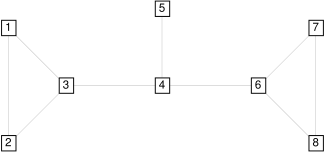
\includegraphics[width=0.75\columnwidth]{\lyxdot \lyxdot /\lyxdot \lyxdot /RO/Notes/graphe}
\par\end{center}

Une \emph{couverture} $C$ de ce graphe est un ensemble de sommets
qui touchent toutes les arêtes, comme par exemple $C:=\left\{ 1,3,4,7,8\right\} $:

\begin{center}
\includegraphics[width=0.75\columnwidth]{\lyxdot \lyxdot /\lyxdot \lyxdot /RO/Notes/graphe-couverture}
\par\end{center}
\begin{example}
On a $8$ petits villages reliés par des routes. En cas d'accident
de la route, on veut que les pompiers puissent intervenir rapidement.
Le prefet impose que lorsqu'une route relie deux villages, il y ait
une caserne de pompier dans au moins l'un des deux villages. Évidemment
le budget est serré, donc on veut construire des casernes de pompier
dans un nombre minimal de villages.

Modélisation: Chaque village est représenté par un sommet du graphe
précédent, les arêtes représentant les routes. Résoudre notre problème
revient à chercher une couverture de taille minimale du graphe.
\end{example}
Un \emph{couplage} $M$ de ce graphe est un ensemble d'arêtes qui
ne se touchent pas, comme par exemple $M:=\left\{ \left\{ 1,3\right\} ,\left\{ 4,5\right\} ,\left\{ 7,8\right\} \right\} $:

\begin{center}
\includegraphics[width=0.75\columnwidth]{\lyxdot \lyxdot /\lyxdot \lyxdot /RO/Notes/graphe-couplage}
\par\end{center}
\begin{example}
On veut loger un groupe de $8$ personnes dans un hotel, avec des
chambres simples et doubles. Pour minimiser les dépenses, on utiliser
le maximum de chambres doubles. D'un autre côté on ne veut pas forcer
deux personnes qui ne se connaissent pas bien à partager une chambre. 

Modélisation: chaque sommet du graphe précédent représente une personne,
et chaque arête relie deux personnes qui se connaissent bien. Résoudre
notre problème revient alors à rechercher un couplage de taille maximale
dans le graphe.\end{example}
\begin{xca}
Montrer que pour un couplage $M$ et une couverture $C$ d'un même
graphe, on a toujours $\left|M\right|\leq\left|C\right|$.
\end{xca}
%

%

%

%

%

%

\solution
\begin{proof}
Comme $C$ est une couverture, chaque arête de $M$ devra être touchée
par au moins un sommet dans $C$. De plus, $M$ étant un couplage,
chaque sommet de $C$ touche au plus une arête de $M$. Donc, on a
bien $\left|M\right|\leq\left|C\right|$.\end{proof}
\begin{problem}
Peut-on trouver $M$ et $C$ de façon à avoir égalité ?
\end{problem}
%

%

%

%

%

\solution

Dans notre exemple, non. Par contre, on va voir que pour certaines
classes de graphe, cela va être vrai: on aura un théorème de dualité
min-max. Comme par hasard, c'est une conséquence de la programmation
linéaire.

On appelle \emph{graphe biparti} un graphe dont on peut partitioner
les sommets en deux paquets $A$ et $B$ de sorte que toutes les arêtes
soient entre $A$ et $B$:

\begin{center}
\includegraphics[width=0.25\columnwidth]{\lyxdot \lyxdot /\lyxdot \lyxdot /RO/Notes/biparti}
\par\end{center}
\begin{xca}
On veut rechercher un couplage maximal du graphe précédent. Montrer
comment on peut résoudre ce problème en utilisant un problème de flot.

Utiliser l'algorithme de Ford-Fulkerson pour le résoudre. 

On appelle cela la \og Méthode du chemin augmentant \fg{}. Pourquoi?
\end{xca}
%

%

%

%

%

\solution

Chaque solution entière $F$ du problème de flot correspond à un couplage
$M$ du graphe biparti (les arêtes sur lesquelles passent une unité),
avec $\left|M\right|=\left|F\right|$. Maximiser le flot revient à
rechercher un couplage de taille max. \emph{Le théorème d'intégralité
nous garanti que Ford-Fulkerson donnera bien une solution optimale
entière}!
\begin{xca}
Prendre maintenant la coupe minimale donnée par l'algorithme de Ford-Fulkerson,
et définir $C$ l'ensemble des sommets $a$ du graphe biparti tels
que:
\begin{itemize}
\item soit $a$ est du côté de la source et $a$ n'est pas dans la coupe.
\item soit $a$ est du côté du puit et $a$ est dans la coupe.\end{itemize}
\begin{enumerate}
\item Que constate-t'on?
\end{enumerate}
\end{xca}
\begin{problem}
Est-ce une coïncidence?\end{problem}
\begin{xca}
Soit $G$ un graphe biparti, $M$ un couplage maximal donné par l'algorithme
de Ford-Fulkerson, et $C$ l'ensemble de sommets obtenu comme ci-dessus.
Montrer que $C$ est une couverture et que $\left|M\right|=\left|C\right|$.$ $
\end{xca}
%

%

%

%

%Écrire la démo

\solution
\begin{thm}
(König-Egerváry) Dans tout graphe biparti, la taille d'un couplage
maximal est égale à la taille d'une couverture minimale.
\end{thm}
C'est une exemple typique où le théorème de dualité de la programmation
linéaire donne un théorème min-max reliant deux problèmes combinatoires
qui ne sont pas en lien direct a priori.
\begin{xca}
Utiliser la méthode du chemin augmentant pour rechercher un couplage
maximal des graphes suivants (on pourra partir du couplage suggéré):

\begin{center}

\includegraphics[width=0.75\columnwidth]{\lyxdot \lyxdot /\lyxdot \lyxdot /RO/Notes/biparti2}
\par\end{center}


\begin{center}
\includegraphics[width=0.75\columnwidth]{\lyxdot \lyxdot /\lyxdot \lyxdot /RO/Notes/couplage2}
\par\end{center}


\begin{center}
\includegraphics[width=0.75\columnwidth]{\lyxdot \lyxdot /\lyxdot \lyxdot /RO/Notes/couplage-berge}
\par\end{center}

\end{xca}

\subsubsection{Dualités chaînes/antichaînes dans les ordres partiels; théorème de
Dilworth}
\begin{problem}
\cite[p. 338]{Chvatal_LP} Problème des visites guidées. Une compagnie
propose $7$ visites guidées dans la journée, notées $a,b,c,d,e,f,g$,
dont les horaires et durées sont fixées. Si une visite (par ex. $a$)
termine suffisament avant une autre (par exemple $c$), le guide de
la première visite peut enchaîner sur la deuxième; on notera alors
$a\rightarrow c$. En l'occurence, voici tous les enchaînements possibles:

$a\rightarrow c,\textrm{ }a\rightarrow d,\textrm{ }a\rightarrow f,\textrm{ }a\rightarrow g,\textrm{ }b\rightarrow c,\textrm{ }b\rightarrow g,\textrm{ }d\rightarrow g,\textrm{ }e\rightarrow f,\textrm{ }e\rightarrow g$.
\begin{itemize}
\item Combien faut-il de guides au minimum dans cet exemple ?
\item Comment trouver le nombre minimum de guides nécessaires dans le cas
général ?
\end{itemize}
\end{problem}
%

%

%

%

%

%

\solution
\begin{defn}
Soit $P=(E,<)$ un ordre partiel. 

Une \emph{chaîne} $C$ de $P$ est un ensemble de sommets de $P$
deux à-deux comparables:
\[
x\in C\textrm{ et }y\in C\textrm{ }\Rightarrow\textrm{ }x<y\textrm{ ou }y<x.
\]


Une \emph{antichaîne} $A$ de $P$ est un ensemble de sommets deux-à-deux
incomparables.

Une \emph{couverture en chaînes} de $P$ est un ensemble $C_{1},\ldots,C_{k}$
de chaînes, de sorte que tout sommet de $P$ est dans une unique chaîne
$C_{i}$.

Une \emph{couverture en antichaînes} de $P$ est un ensemble $A_{1},\ldots,A_{k}$
d'antichaînes, de sorte que tout sommet de $P$ est dans une unique
antichaîne $A_{i}$.\end{defn}
\begin{xca}
Trouver dans l'ordre partiel $P$ précédent:
\begin{enumerate}
\item Une chaîne de taille maximale
\item Une antichaîne de taille maximale
\item Une couverture en chaînes de $P$ de taille minimale
\item Une couverture en antichaînes de $P$ de taille minimale
\end{enumerate}
Que remarquez vous ?
\end{xca}
%

%

%

\solution

Y-aurait-il un théorème min-max reliant la taille de la plus grande
chaîne et la taille de la plus petite couverture en antichaînes ?
Et un autre reliant la taille de la plus grande antichaîne et celle
de la plus petite couverture en chaînes ?
\begin{xca}
Soit $P$ un ordre partiel quelconque.
\begin{enumerate}
\item Soit $C$ une chaîne de $P$ et $A_{1},\ldots,A_{k}$ une couverture
de $P$ en antichaînes.


Montrer que $\left|C\right|\leq k$.

\item Soit $A$ une antichaîne de $P$ et $C_{1},\ldots,C_{k}$ une couverture
de $P$ en chaînes.


Montrer que $\left|A\right|\leq k$.

\end{enumerate}
\end{xca}
\begin{prop}
Soit $P$ un ordre partiel. La taille de la plus grande chaîne de
$P$ est égale à la taille de la plus petite couverture en antichaînes
de $P$.\end{prop}
\begin{xca}
Prouvez-le!
\end{xca}
%

%

%

%

%

\solution

Le théorème dans l'autre sens est plus difficile et bien plus profond.
Il n'y a pas de construction élémentaire de l'antichaîne et de la
couverture en chaîne idoine. On va en fait se ramener au théorème
de dualité de la programation linéaire (surprise).
\begin{thm}
(Dilworth) Soit $P$ un ordre partiel. La taille de la plus grande
antichaîne de $P$ est égale à la taille de la plus petite couverture
en chaînes de $P$.\end{thm}
\begin{proof}
On note $n$ le nombre de sommets de $P$. 

Choisir une couverture en chaîne de $P$ est équivalent à sélectionner
un certain nombre d'arcs dans $P$, de sorte que chaque sommet ait
au plus un arc sortant de sélectionné, et un arc rentrant de sélectionné. 

Remarque: s'il y a $k$ chaînes, il y a $n-k$ arcs sélectionnés.

Cela ressemble à un problème de couplage maximal dans un graphe biparti.

On construit un graphe biparti $B$ dans lequel chaque sommet $x$
de $P$ est dupliqué en $(x,1)$ et $(x,2)$. 

Chaque fois que $x<y$ dans $P$, on relie $(x,1)$ et $(y,2)$.

Qu'est-ce qu'un couplage dans $B$?

Un ensemble d'arcs de $P$ vérifiant exactement les conditions voulues.

Une couverture de $P$ en $k$ chaînes correspond à un couplage de
$B$ de taille $n-k$.

Prenons une couverture de $P$ de taille $k$ minimale.

Cela donne un couplage de taille max $n-k$ de $B$.

Le théorème min-max pour les graphes bipartis indique qu'il y a une
couverture de $B$ de même taille: $n-k$ sommets de $B$ qui touchent
tous les arcs.

Dans $P$ cela correspond à au plus $n-k$ sommets qui touchent tous
les arcs.

Soit $A$ l'ensemble des sommets restants qui est de taille au moins
$k$.

Il ne peut pas y avoir d'arcs entre deux sommets de $A$. 

Conclusion: $A$ est une antichaîne de taille au moins $k$.\end{proof}
\begin{xca}
Suivez le déroulement de la preuve sur l'ordre partiel précédent.
\end{xca}

\subsubsection{Problème des mines à ciel ouvert}
\begin{problem*}
Des études géologiques ont permis de déterminer précisément la nature
du sous-sol, et l'emplacement des gisements orifères à l'endroit ou
l'on a décidé de creuser une mine à ciel ouvert. Certains gisements
sont profonds, et il n'est pas clair qu'il soit rentable d'excaver
tout le sol au-dessus pour y accéder.

Modèle: le sous-sol a été délimité en un certain nombre de blocs.
Pour chaque bloc $i$, on connaît le coût $C_{i}$ d'excavation, et
le profit $P_{i}$ que l'on peut escompter de son traitement.

Au final, on associe à chaque bloc $i$ la quantité $w_{i}=C_{i}-P_{i}$.
Si l'on ne considère pas les autres blocs, il est rentable de creuser
$i$ si et seulement si $w_{i}<0$.

On veut déterminer quels blocs on doit creuser pour maximiser le profit
total $-\sum_{i}w_{i}$ (ou autrement dit minimiser $\sum_{i}w_{i}$).

Maintenant, il y a des contraintes supplémentaires: si un bloc $i$
est sous un bloc $j$, on ne peux pas creuser $i$ sans creuser $j$!

On introduit un ordre partiel, de sorte que $i<j$ si pour creuser
$i$ on doit creuser $j$.

Comme on le verra, la forme des blocs, et le type d'ordre partiel
n'est pas relevant.\end{problem*}
\begin{example*}
On considère le sous-sol suivant:
\end{example*}
Comment modéliser notre problème sous forme de problème de flot max
?

La modélisation des contraintes de précédences est un peu astucieuse!

On introduit le réseau suivant:

C'est la remarque suivante qui va faire marcher la machine:
\begin{rem*}
Soit $C$ une coupe. 

S'il existe deux blocs $i<j$, avec $i\in C$ et $j\in C$, alors
$C$ est de capacité infinie.

La réciproque est vraie.
\end{rem*}
Les coupes de capacité finie sont en correspondance avec les coupes
respectant les contraintes.

Maintenant, on peut vérifier que la capacité d'une coupe finie vaut
exactement

\[
\sum_{i\in C,\textrm{ }i\textrm{ bloc non rentable}}w_{i}-\sum_{i\not\in C,\textrm{ }i\textrm{ bloc rentable}}w_{i}.
\]


Quitte à rajouter le terme constant $\sum_{i,\textrm{ }i\textrm{ bloc}}w_{i}$,
on est en train de calculer le profit lorsque l'on enlève les blocs
$i$ avec $i\in C$.

Résumé: Soit $I$ un ensemble de blocs, et $C$ la coupe $\left\{ s\right\} \cup I$.
\begin{itemize}
\item Si $I$ ne satisfait pas les contraintes, la capacité de $C$ est
infinie.
\item Si $I$ satisfait les contraintes, la capacité de $C$ est l'opposé
du profit.
\end{itemize}
Maximiser le profit revient à trouver une coupe min.
\begin{rem*}
En termes pédants: on peut résoudre par un algorithme de flot le problème
de trouver une section finale de poids minimal dans un ordre partiel.
\end{rem*}

\section{Synthèse}

Plusieurs modèles généraux pour faire de l'optimisation:
\begin{enumerate}
\item Programmation linéaire

\begin{enumerate}
\item Algorithme du simplexe\\
Efficace en pratique (quasiment linéaire), non polynomial en théorie
\item Algorithme de l'élipsoide\\
Polynomial, mais non efficace en pratique
\item Méthode des points intérieurs\\
Plus ou moins efficace que le simplexe selon les cas
\item Théorème de dualité $\Longrightarrow$ Certification, optimisation,
coûts marginaux, \ldots{}
\item Mais: solutions dans $\mathbb{Q}$
\end{enumerate}
\item Problèmes de flots

\begin{enumerate}
\item Algorithme de Ford-Fulkerson\\
Polynomial $O(n^{3})$. Plus efficace que le simplexe.
\item Théorème de dualité (flots/coupes)
\item Théorème d'intégralité\\
 $\Longrightarrow$ Algorithmes et théorèmes min-max sur des problèmes
discrets.
\end{enumerate}
\item Réseaux de transports

\begin{enumerate}
\item Algorithme du simplexe pour les réseaux
\item Théorème de dualité (coûts marginaux)
\item Théorème d'intégralité
\end{enumerate}
\end{enumerate}
\begin{thebibliography}{1}
\bibitem{Chvatal_LP}V.~Chvatal. Linear Programming.

\bibitem{Vanderbie_LPFE}R.~Vanderbie. Linear Programming; Foundations
and Extensions. \url{http://www.princeton.edu/~rvdb/LPbook/index.html}

\bibitem{LP_FAQ}Linear Programming FAQ \url{http://rutcor.rutgers.edu/~mnk/lp-faq.html}

\bibitem{Wikipedia}\url{http://en.wikipedia.org/wiki/Linear_programming}\end{thebibliography}

\end{document}
